% Section 7: choosing between mode imputation and the "Missing" category, with the two house-price columns placed
% at the end they reach. GarageQual: 5.5% missing, TA 95.1% of known values. FireplaceQu: 47.3% missing, Gd 49.1%
% against TA 40.6%. MCAR is checked by comparing the target for gap rows and mode rows (Section 5.2).
\documentclass[tikz,border=8pt]{standalone}
% Shared look for every TikZ diagram. Load with % Shared look for every TikZ diagram. Load with % Shared look for every TikZ diagram. Load with \input{../../tools/tikz-style.tex}
\usepackage[T1]{fontenc}
\usepackage{lmodern}
\renewcommand{\sfdefault}{lmr}  % diagrams use the same serif as the text
\usetikzlibrary{arrows.meta, positioning, shapes.geometric, calc, fit, backgrounds}
\definecolor{cblue}{HTML}{4C78A8}
\definecolor{corange}{HTML}{F58518}
\definecolor{cgreen}{HTML}{54A24B}
\definecolor{cred}{HTML}{E45756}
\definecolor{cpurple}{HTML}{B279A2}
\definecolor{cgrey}{HTML}{6B6B6B}
\tikzset{
  every picture/.style={font=\sffamily, line width=1.2pt},
  box/.style={draw=#1, fill=#1!12, rounded corners=4pt, align=center, inner sep=7pt, minimum height=1.1cm},
  box/.default=cgrey,
  arrow/.style={-{Stealth[length=3mm]}, draw=cgrey, line width=1.4pt},
  title/.style={font=\sffamily\bfseries\Large},
  note/.style={font=\sffamily\small, text=cgrey, align=center},
}
\AtBeginDocument{\hyphenpenalty=10000 \exhyphenpenalty=10000}

\usepackage[T1]{fontenc}
\usepackage{lmodern}
\renewcommand{\sfdefault}{lmr}  % diagrams use the same serif as the text
\usetikzlibrary{arrows.meta, positioning, shapes.geometric, calc, fit, backgrounds}
\definecolor{cblue}{HTML}{4C78A8}
\definecolor{corange}{HTML}{F58518}
\definecolor{cgreen}{HTML}{54A24B}
\definecolor{cred}{HTML}{E45756}
\definecolor{cpurple}{HTML}{B279A2}
\definecolor{cgrey}{HTML}{6B6B6B}
\tikzset{
  every picture/.style={font=\sffamily, line width=1.2pt},
  box/.style={draw=#1, fill=#1!12, rounded corners=4pt, align=center, inner sep=7pt, minimum height=1.1cm},
  box/.default=cgrey,
  arrow/.style={-{Stealth[length=3mm]}, draw=cgrey, line width=1.4pt},
  title/.style={font=\sffamily\bfseries\Large},
  note/.style={font=\sffamily\small, text=cgrey, align=center},
}
\AtBeginDocument{\hyphenpenalty=10000 \exhyphenpenalty=10000}

\usepackage[T1]{fontenc}
\usepackage{lmodern}
\renewcommand{\sfdefault}{lmr}  % diagrams use the same serif as the text
\usetikzlibrary{arrows.meta, positioning, shapes.geometric, calc, fit, backgrounds}
\definecolor{cblue}{HTML}{4C78A8}
\definecolor{corange}{HTML}{F58518}
\definecolor{cgreen}{HTML}{54A24B}
\definecolor{cred}{HTML}{E45756}
\definecolor{cpurple}{HTML}{B279A2}
\definecolor{cgrey}{HTML}{6B6B6B}
\tikzset{
  every picture/.style={font=\sffamily, line width=1.2pt},
  box/.style={draw=#1, fill=#1!12, rounded corners=4pt, align=center, inner sep=7pt, minimum height=1.1cm},
  box/.default=cgrey,
  arrow/.style={-{Stealth[length=3mm]}, draw=cgrey, line width=1.4pt},
  title/.style={font=\sffamily\bfseries\Large},
  note/.style={font=\sffamily\small, text=cgrey, align=center},
}
\AtBeginDocument{\hyphenpenalty=10000 \exhyphenpenalty=10000}

\begin{document}
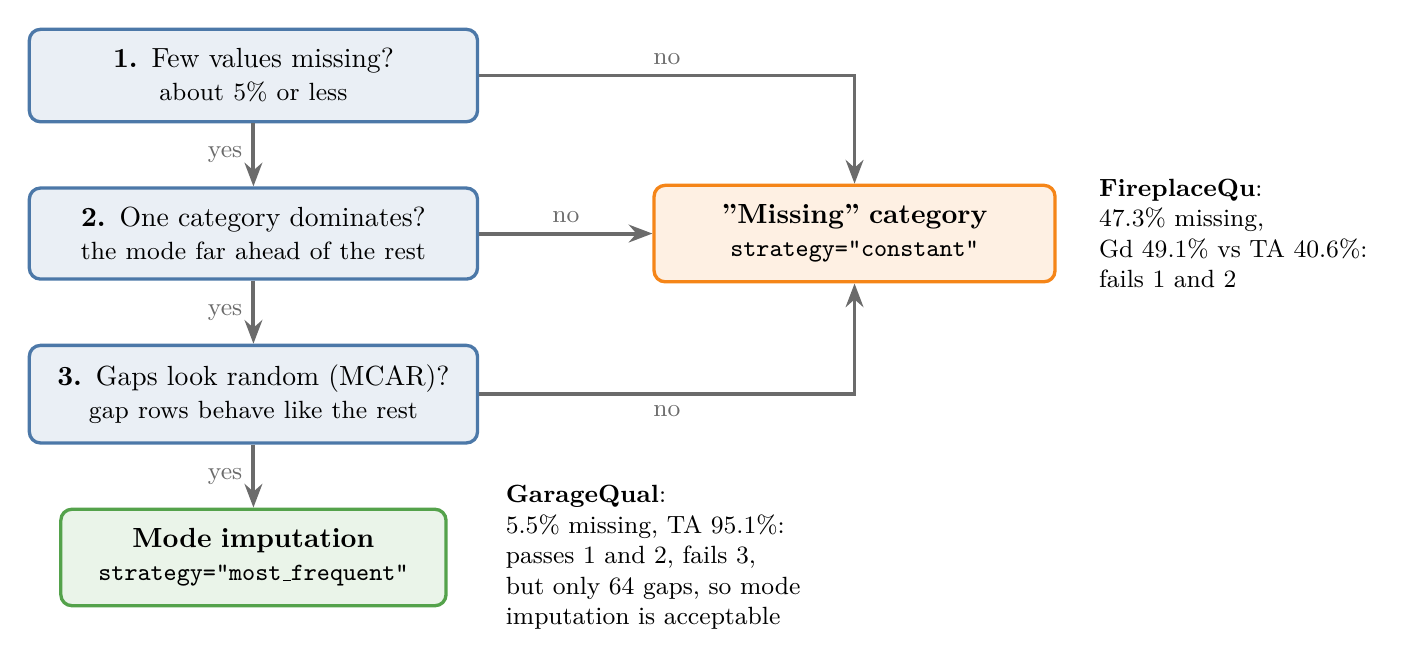
\begin{tikzpicture}[node distance=0.8cm and 1.2cm, q/.style={box=cblue, text width=5.2cm}]
  \node[q] (q1) {\textbf{1.} Few values missing?\\\small about 5\% or less};
  \node[q, below=of q1] (q2) {\textbf{2.} One category dominates?\\\small the mode far ahead of the rest};
  \node[q, below=of q2] (q3) {\textbf{3.} Gaps look random (MCAR)?\\\small gap rows behave like the rest};
  \node[box=cgreen, text width=4.4cm, below=of q3] (mode) {\textbf{Mode imputation}\\\small \texttt{strategy="most\_frequent"}};
  \node[box=corange, text width=4.6cm, right=2.2cm of q2] (miss) {\textbf{"Missing" category}\\\small \texttt{strategy="constant"}};
  \draw[arrow] (q1) -- node[note, left] {yes} (q2);
  \draw[arrow] (q2) -- node[note, left] {yes} (q3);
  \draw[arrow] (q3) -- node[note, left] {yes} (mode);
  \draw[arrow] (q1.east) -| node[note, pos=0.25, above] {no} (miss.north);
  \draw[arrow] (q2.east) -- node[note, above] {no} (miss.west);
  \draw[arrow] (q3.east) -| node[note, pos=0.25, below] {no} (miss.south);
  \node[note, text width=3.6cm, right=0.4cm of miss, text=black, align=left] (f) {\textbf{FireplaceQu}:\\47.3\% missing,\\Gd 49.1\% vs TA 40.6\%:\\fails 1 and 2};
  \node[note, text width=5.4cm, right=0.6cm of mode, text=black, align=left] (g) {\textbf{GarageQual}:\\5.5\% missing, TA 95.1\%:\\passes 1 and 2, fails 3,\\but only 64 gaps, so mode\\imputation is acceptable};
  
\end{tikzpicture}
\end{document}
